\documentclass{article}
\usepackage{hyperref}
\hypersetup{
    colorlinks=true,
    linkcolor=black,
    filecolor=black,      
    urlcolor=black,
    pdftitle={Overleaf Example},
    pdfpagemode=FullScreen,
    }
\usepackage[utf8]{inputenc}
\usepackage{geometry}
 \geometry{
 a4paper,
 total={170mm,257mm},
 left=20mm,
 top=20mm,
 }
\usepackage{graphicx}
\usepackage{titling}
\usepackage{subcaption}
\usepackage{caption}

 \title{\huge \textbf{Sport video analysis for billiard matches} \newline \Large Computer Vision Project - June/July 2024
}
\author{Artico Giovanni \\ \href{mailto:giovanni.artico@studenti.unipd.it}{giovanni.artico@studenti.unipd.it} \\ \\
        Giacomin Marco \\  \href{mailto:marco.giacomin@studenti.unipd.it}{marco.giacomin@studenti.unipd.it} \\ \\
        Toffolon Mattia \\ \href{mailto:mattia.toffolon@studenti.unipd.it}{mattia.toffolon@studenti.unipd.it}}
\date{}
 
\usepackage{fancyhdr}
% \fancypagestyle{plain}{%  the preset of fancyhdr 
%     \fancyhf{} % clear all header and footer fields
%     \fancyfoot[L]{\thedate}
%     \fancyhead[L]{Computer Vision AY 2023/2024}
%     \fancyhead[R]{\theauthor}
% }
\makeatletter
% \def\@maketitle{%
%   \newpage
%   \null
%   \vskip 1em%
%   \begin{center}%
%   \let \footnote \thanks
%     {\LARGE \@title \par}%
%     \vskip 1em%
%     %{\large \@date}%
%   \end{center}%
%   \par
%   \vskip 1em}
% \makeatother

\usepackage{lipsum}  

\begin{document}

\maketitle
\vspace{10mm}
\tableofcontents

\newpage

\section{Introduction}
\section{Introduction}

In this first section, the main purpose of the project and how the developed project has been evaluted will be presented.


\subsection{Problem specifics}
The aim of this project is to develop a computer vision system for analyzing video footage of various “Eight Ball”
billiard game events by providing high-level information about the status of the match for each video frame in the form of a 
2D top-view minimap.
\newline
More in detail, the system should be able to:
\begin{itemize}
    \item Recognize and localize all the balls inside the playing field, distinguishing them based on their category (1-the
    white “cue ball”, 2-the black “8-ball”, 3-balls with solid colors, 4-balls with stripes);
    \item Detect all the main lines (boundaries) of the playing field;
    \item Segment the area inside the playing field boundaries detected in point 2 into the following categories: 1-the
    white “cue ball”, 2-the black “8-ball”, 3-balls with solid colors, 4-balls with stripes, 5-playing field;
    \item Represent the current state of the game in a 2D top-view visualization map, to be updated at each new frame
    with the current ball positions and the trajectory of each ball that is moving;
    \item Create a modified version of each video in which the generated 2D maps are 
    overlayed on a corner of the respective frames.
\end{itemize}

\begin{flushleft}
The available dataset consists of 10 folders each one corresponding to a different game event and containing:
\end{flushleft}
\begin{itemize}
    \item a \verb|.mp4| file corresponding to the event video;
    \item a \verb|.png| file corresponding to the first frame of the video;
    \item a \verb|.png| file corresponding to the last frame of the video.
\end{itemize}

% \begin{flushleft}
% For each game event video frame, the developed system is able to produce: 
% \end{flushleft}
% \begin{itemize}
%     \item a table segmentation mask;
%     \item a vector of \verb|Ball| structs that, as it will be better explained later, are composed by a bounding box (\verb|Rect| object)
%     defined by 4 parameters [x, y, width, height], where (x,y) are the top-left corner coordinates and width and height
%     are the bounding box main dimensions, and a ball type (\textit{CUE} = 1, \textit{EIGHT} = 2, \textit{SOLID} = 3,
%     \textit{STRIPED} = 4);
%     \item a ball segmentatation mask derived from the produced bounding boxes;
%     \item a 2D top-view visualization map representing the balls typology and current positions in the table, along with the trajectories of the balls
%     that have moved in the video so far (video frames upto the current one).
% \end{itemize}

% \begin{flushleft}
% For each game event video instead, the developed system is able to produce a modified version of the selected video in which the generated 2D maps are 
% overlayed to the respective frames.
% \end{flushleft}



\subsection{Performance evaluation}
To evaluate the system performance, the metrics that should be adopted are:
\begin{itemize}
    \item mean Average Precision (mAP);
    \item mean Intersection over Union (mIoU).
\end{itemize}
\begin{flushleft}
Further insights on how these values were computed and used can be found in Section \ref{sec:performance}.
\end{flushleft}


\subsection{Sub-task identification}
To develop the system, the problem was divided into the following sub-tasks:
\begin{itemize}
    \item Table segmentation;
    \item Table sides recognition;
    \item Balls localization and segmentatation;
    \item Balls identification;
    \item Balls tracking;
    \item Map rendering;
    \item System performance evaluation.
\end{itemize}


\section{Table Segmentation (Artico Giovanni)}
The following assumptions were made for the segmentation of the table
\begin{itemize}
    \item the table is a uniform color and is a prevalent part of the image
    \item the table is centered (or close to being centered) in the image
\end{itemize}

It is going to be apparent the reason for these when the full algorithm for
the segmentation of the table is explained.
The first thing that was to be found was a rough segmentation of the table,
as finding the lines with only the Canny-transform of the full image would 
be problematic, as the strongest lines in the image are not only the table
fabric, but also the table itself and various other things in the image.
The initial approach was to use Otsu's thresholding, as the table is a uniform
color, therefore it is sensible to assume it would be thresholded the same
way throughout. This proved unfruitful, as the segmentation was too rough.
The second approach was to use kmeans clustering, in particular exploiting the
adaptability of the algorithm in order to use spatial features too to improve
the segmentation, as we assume the table is a continuous entity. Out of the k clusters obtained the most centered one was picked.
The segmentation obtained was fairly precise but contained multiple disconnected
components, however we can consider the table the biggest and pick it, in particular
before doing this operation open is applied in order to remove weakly connected objects.
the k (empirically) chosen was 3, as 2 lead to undersegmentation of the image and 4 to oversegmentation.
The resulting segmentation is precise in most cases, but given the nature of kmeans on some
images it fails, as it clusters some unrelated parts of the table with the fabric, due,
for example, to lighting.
For this reason further processing was required, given we have obtained a rough mask of
the table we now obtain the mean color of the image in the pixels where the mask is non-zero.
After this we use a color thresholding by distance from the mean and the same way we 
did before to obtain the largest connectedcomponent. In particular thresholding on the hue
is the most robust, in particular a low distance, 5, was chosen, but similar distances give similar
results.\par
after having obtained this result dilation is applied in order to remove some noise from the mask,
for example balls or other objects. Afterwards the hough transform is used to find the lines, 
with a threshold in order to remove similar lines.
The vertices of the table are found using the equations from \href{https://en.wikipedia.org/wiki/Line\%E2\%80\%93line\_intersection}{wikipedia}.
It is to note that the last frame is used for such frame as most of the time it doesn't contain the player in the table, being at the end of
a turn.

\begin{figure}
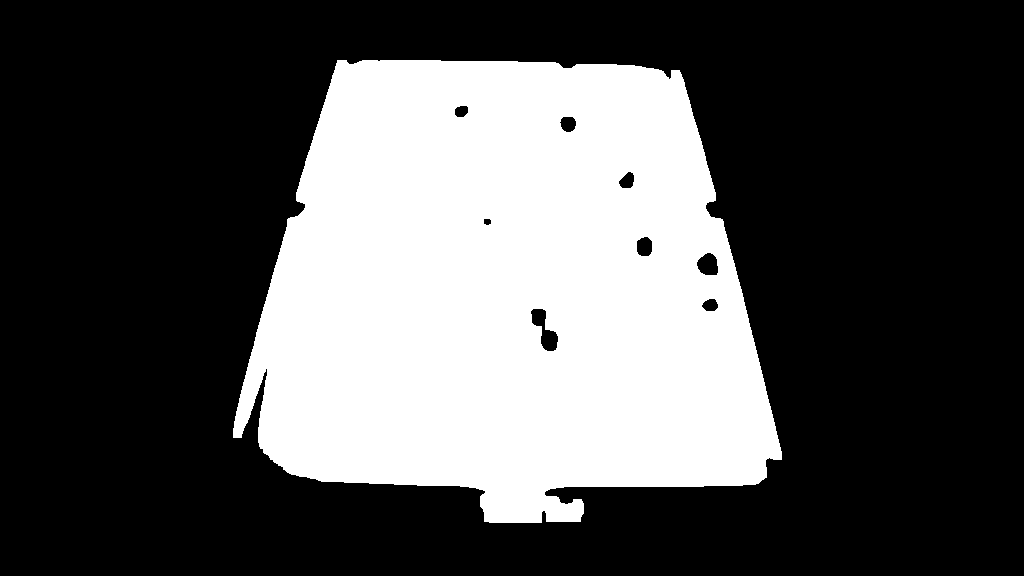
\includegraphics[width=0.6\textwidth]{./imgs/kmeans_cluster.png}
\caption{initial kmeans clustering result}
\end{figure}
\begin{figure}
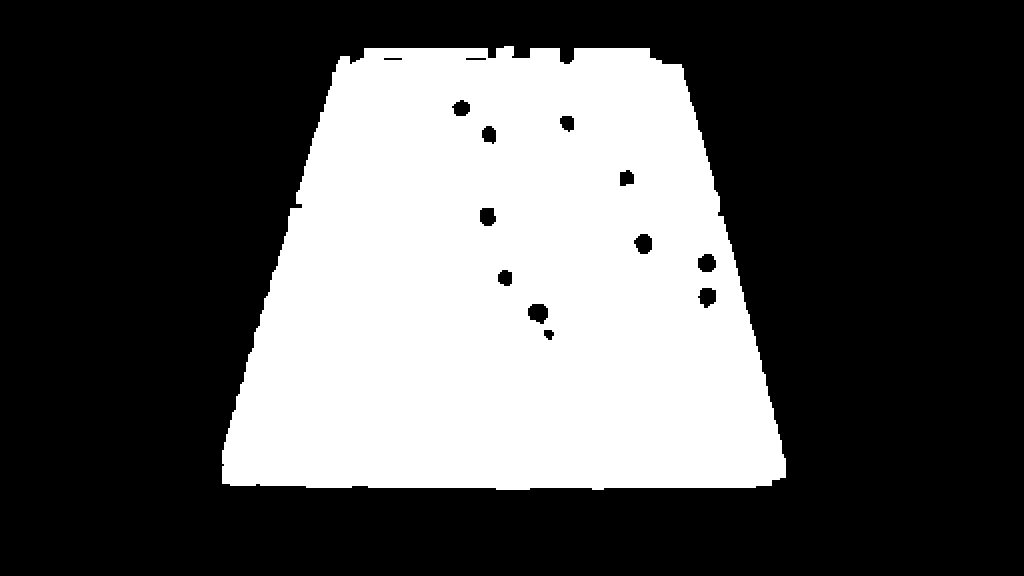
\includegraphics[width=0.6\textwidth]{./imgs/color_cluster.png}
\caption{final color clustering result}
\end{figure}


\section{Table Side Recognition (Artico Giovanni)}
\section{Table Side Recognition}

The points are ordered from the upper-left-most point clockwise, but this doesn't give
any information on how the sides are ordered. It is unfortunately impossible (or out of my
mathematical capabilities) to find any meaningful geometrical relation between the sides
given the perspective deformations in some cases. The only feature we can go off of is the 
holes in the middle of the longer sides. The first operation was to obtain the rotated
rectangles containing the sides of the pool table, with a small width as to avoid 
keeping in the images unneeded information.\par 
Multiple approaches were tested to distinguish the two types of sides. The first was 
to use features (such as harris corners or SIFT), as intuitively they should appear 
on the holes and not on uniform sides as they should be classified as edges. This didn't
work, as the features and corners detected most of the time were spread throughout the 
considered sides most of the times as shown in \ref{fig:sift}.\par
The next approach was to try template matching between 3 different segments of the side image,
as the center contains a hole which should make the match significantly worse than
between the left and right segment. This does not work for two reasons:
\begin{itemize}
    \item because of the perspective the hole can appear in a part of the segment of the image that is not the center one
    \item because of the illumination and small imprecisions on the table segmentation the matching would fail even on the segments which should result similar
\end{itemize}
both of these are shown in figure \ref{fig:difficultside}.
\par
Ultimately the way to recognize the sides was the following:
\begin{enumerate}
    \item apply the Canny tranform on the initial image
    \item extract the rectangles from the image
    \item rotate the rectangles so that they are all horizontal
    \item apply sobel on the x-axis shown in image \ref{fig:sidestabol}
    \item sum over the contribution on the middle two quarters (as to avoid considering the corner holes) of the rectangles (normalized over the number of pixels contained in each)
    \item determine the longer sides by the highest contributions
\end{enumerate}
This works because of the nature of the edges on the sides: on shorter sides there
are mostly parallel lines, instead on longer there are strong edges orthogonal to the direction of the sides given by the holes.

\begin{figure}
    \centering
    \begin{subfigure}[b]{\textwidth}
    
\includegraphics[width=\textwidth]{./imgs/sobel_long_side.png}
    \caption{processed rectangle of a long side}\par
    \end{subfigure}\vspace{10pt}
    \begin{subfigure}[b]{\textwidth}
    
\includegraphics[width=\textwidth]{./imgs/sobel_short_side.png}
    \caption{processed rectangle of a long side}
    \end{subfigure}
    \caption{output of the processing of the sides}
    \label{fig:sidestabol}
\end{figure}
\begin{figure}
    \centering
    \begin{subfigure}[b]{\textwidth}
    
\includegraphics[width=\textwidth]{./imgs/bad_side_illumination_change.png}
    \caption{extreme illumination change in the  center of the side}\par
    \end{subfigure}\vspace{10pt}
    \begin{subfigure}[b]{\textwidth}
    
\includegraphics[length=\textwidth, angle=90]{./imgs/bad_side_warp.png}
    \caption{not centered hole}
    \end{subfigure}
    \caption{examples of difficulties in side recognition}
    \label{fig:difficultside}
\end{figure}
\begin{figure}
    \centering
    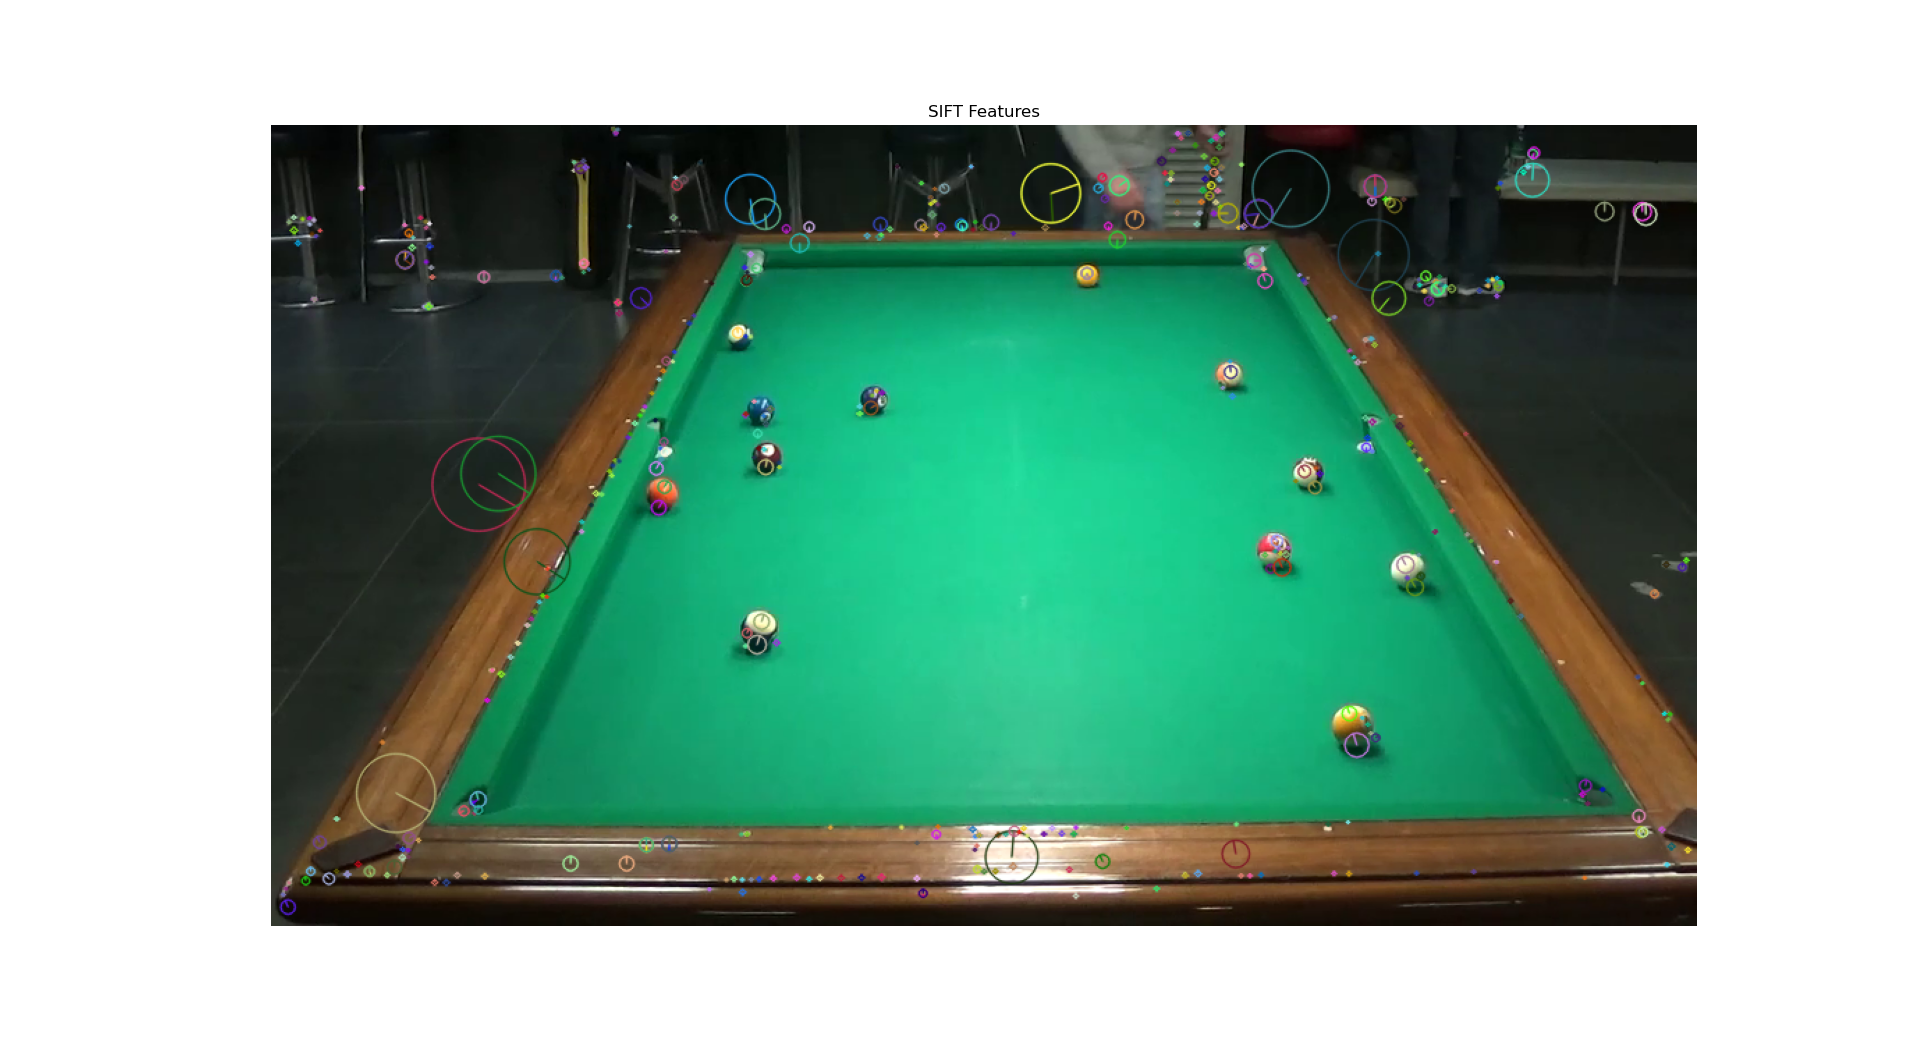
\includegraphics[width=0.5\textwidth]{./imgs/sift.png}
    \caption{Sift features in a sample image}
    \label{fig:sift}
\end{figure}


\section{Ball Localization and Segmentation (Toffolon Mattia)}
\section{Balls Localization and Segmentation}

To solve the ball localization and segmentation sub-tasks the following algorithm was implemented.
The latter goes through the following three major steps:
\begin{enumerate}
    \item Region proposals generation
    \item False positive filtering
    \item Bounding boxes refinement
\end{enumerate}

Before starting with the actual algorithm presentation, a few consideration must be made.
Exclusively for this project part, the used first video frame is the one contained in the given "frames" folder, which is different
from the one taken directly from the video using OpenCV due to compression factors. This choice was made because better system performance relative to 
ball localization and segmentation were obtained using the former.

Furthermore, this section only accurately covers the Ball Localization task solution, showing how the final set of bounding boxes is obtained.
The adopted solution for the Balls Segmentation task, simply consists in creating a mask obtained by fitting a circle inside the found bounding boxes.
As it will explained, the boxes were constrained to be squared, so this operation was trivial.


\subsection{Region proposals generation}
This first step of the algorithm aims to generate regions of interest that will very likely 
contain a ball. The idea behind this step is to find circular regions in the image and create for each one of them
a bounding box to contain it. To do this, the Hough Transform algorithm applied to circles was adopted
(\textit{HoughCircles()} in OpenCV).

Although, the algorithm wasn't applied directly on the grayscale version of the image since
this would have lead to a great number of false positives and false negatives. 
The false positive origin from circles in the image coming from objects in the table different from the balls.
False negatives instead are caused by some balls having almost exactly the same grayscale pixel intensity value of the table cloth,
making \verb|HoughCircles| unable to detect them.
For this algorithm step, the aim is to nullify the number of false negatives, ensuring that every ball is covered by bounding box.
The removal of false positives from the set of found boxes is covered by the second step of the algorithm.

A pre-processing that highlights the balls in the table was needed in order to ease the detection via \verb|HoughCircles|.
The first try involved \verb|K-means| clustering in the color space. Ideally, with parameter \verb|K| big enough, table and balls should have been
clustered in different sets given the differences in color. Although, given the great number of table cloth color variations caused by major illumination
differences between table areas, a great number of found centroids belonged to the table instead of the balls, leading to many balls being clustered
into table regions. Given this result, the second try involved associating each pixel with the closest center (Euclidead distance) in the color space given a pre-defined sets of centers.
The latters were manually defined as ideal ball colors and estimated table cloth color (this estimation is explained later in this section).
In this way it was possibile to correctly clusterize all table pixels but with the inconvenience of including some balls to the table cluster, since the estimated
cloth color was closer to the pixel intensity that the respective ideal ball color. This problem is caused mostly by the fact that the illumination condition of the balls
makes the ball much darker than it actually is. To counteract this issue, additional centers were added to the set exploiting the "value" channel of the HSV enconding
the generate darker variations of the ball colors. Despite the higher quality of the newly found found clustering, a few false negatives were still generated.
The cause of this issue was still the extreme color similary between some balls and table cloth. More specifically, if a dark green ball is located in a poorly lit 
region of a green table, the ball became undetectable. Same reasoning for the blue case.

The best image pre-processing found with respect to the aim of this algorithm step, proved to be the following.
Firstly, the mask obtained through the table segmentation was used to isolate the table in the image
in order to constrain HoughCircles to detect circles only inside the table (Figure \ref{fig:masking}). \\
\begin{figure}[h!]
    \centering
    \begin{subfigure}[b]{0.45\textwidth}
        \centering
        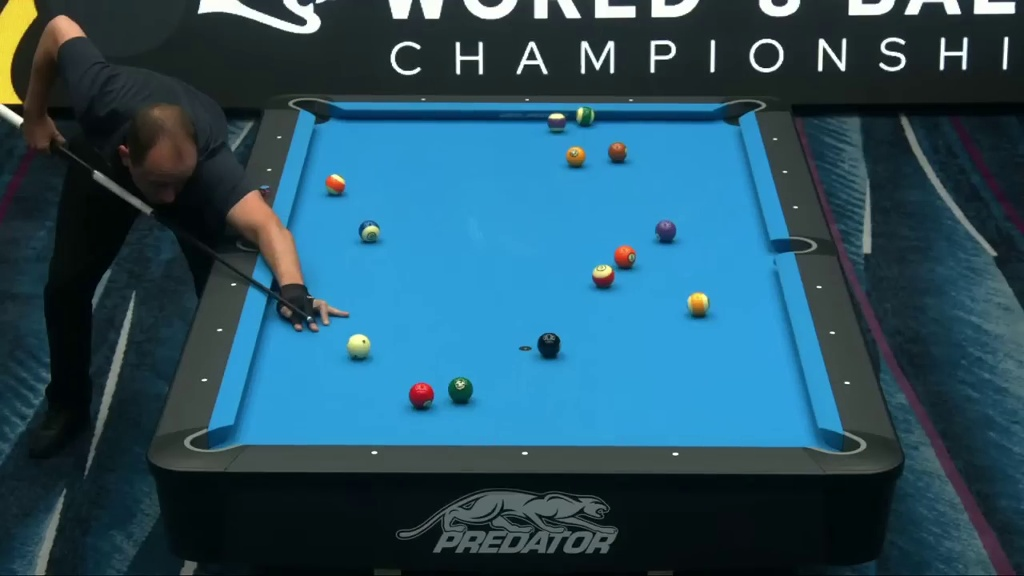
\includegraphics[width=\textwidth]{imgs/ball_localization/original.jpg}
        \caption{Original image}
    \end{subfigure}
    \hspace{0.05\textwidth}
    \begin{subfigure}[b]{0.45\textwidth}
        \centering
        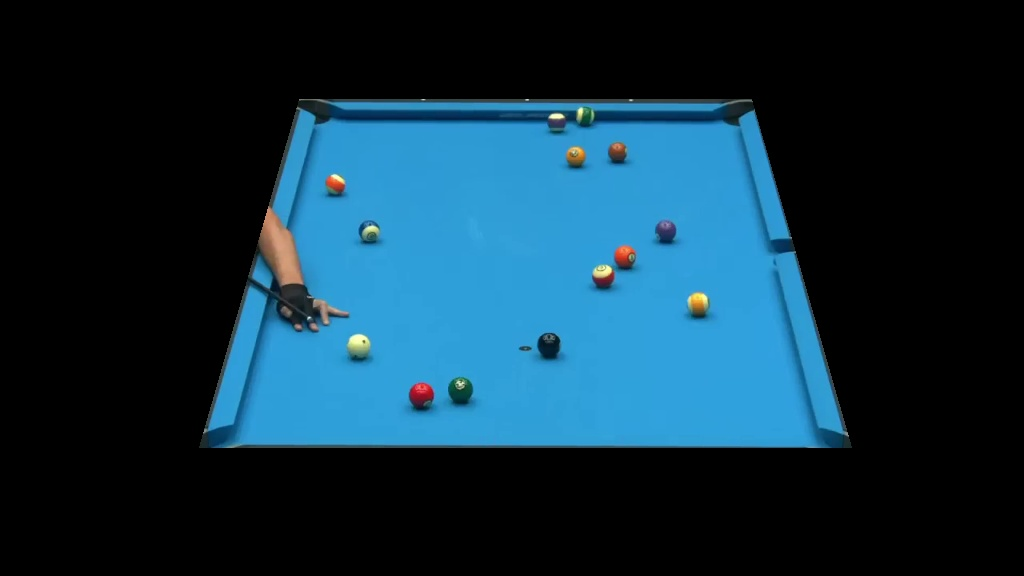
\includegraphics[width=\textwidth]{imgs/ball_localization/masked.jpg}
        \caption{Masked image}
    \end{subfigure}
    \caption{Removal of regions outside of the table one (game1\_clip4)}
    \label{fig:masking}
\end{figure}

Secondly, to ease to detection of circles relative to balls in the table, the following local operation applied to the image pixels
proved to be very effective. Since the table area is mostly empty, the pixel intensity of the table
was evaluated as the mean intensity of non-zero value pixels in the masked image. After this, each non-zero pixel
was set to the absolute value of the difference between the pixel intensity and the evaluated table one.
In this way, all table pixels were set at a value close to zero and instead the balls at a higher intensity
across at least one of the three channels due to differences from the table.
This results in an alternative version of the image in which the table is darker and the transition
between table and balls is much more marked (Figure \ref{fig:subtraction}). \\
\begin{figure}[h!]
    \centering
    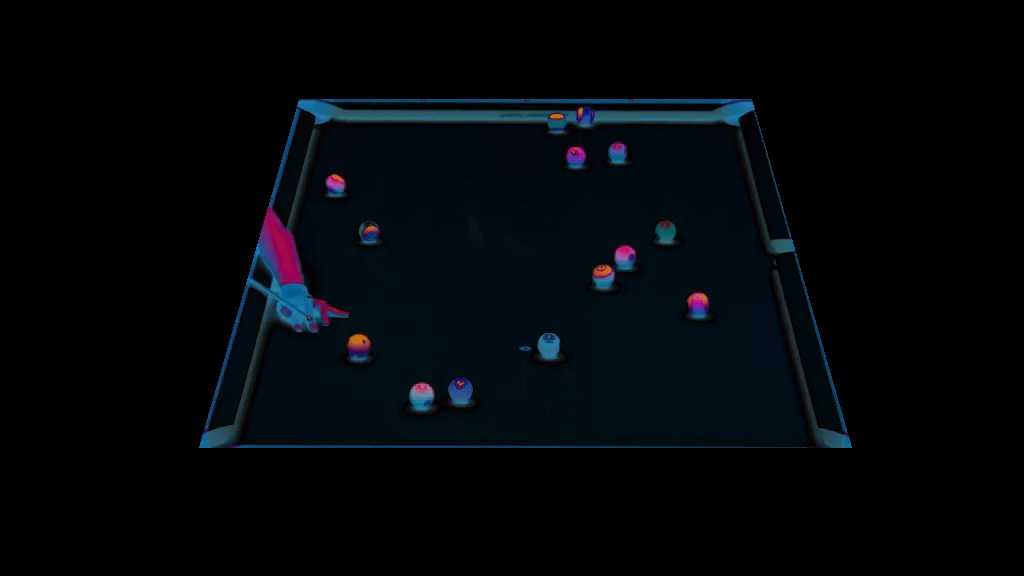
\includegraphics[width=0.85\textwidth]{imgs/ball_localization/subtracted.jpg}
    \caption{Custom local operation is applied to non-zero value pixels (game1\_clip4)}
    \label{fig:subtraction}
\end{figure}

After this, the image was converted to grayscale and HoughCircles was used on it with a general range
of parameters (Method: \verb|Hough_Gradient|, Radius range: 5-15, Distance between circles: \verb|img.rows|/32, Accumulator threshold: 12).
Working only with the BGR version of the image proved to be unsufficient to find all balls because of the 
poor attention to illumination changes of the table color that made impossibile to detect some balls. To solve this issue
the previous steps are performed a second time on the HSV version of the image in order to focus more on 
the colors brightness (value channel). Figure \ref{fig:circles} illustrates an example of these two detections. \\
\begin{figure}[h!]
    \centering
    \begin{subfigure}[b]{0.85\textwidth}
        \centering
        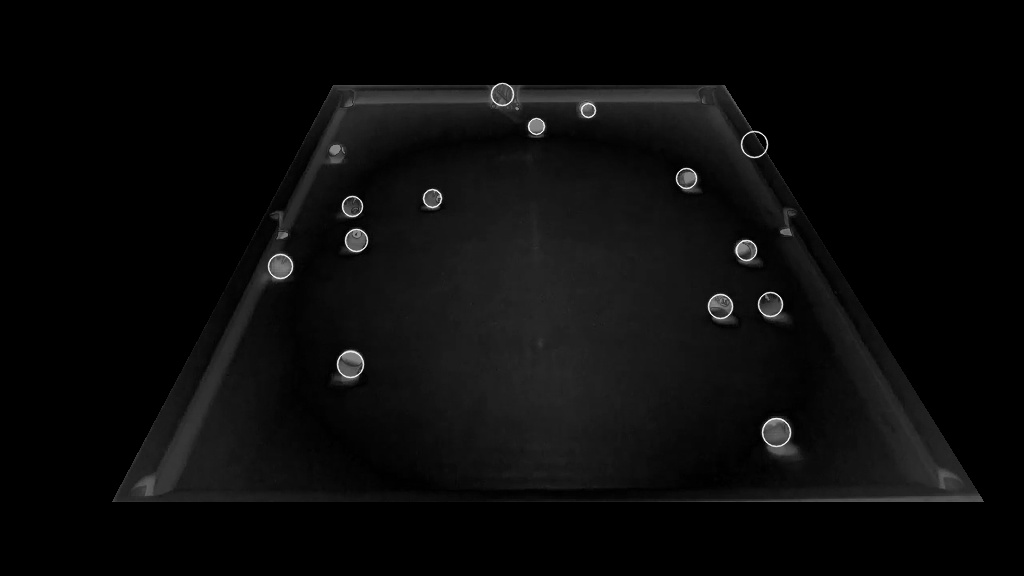
\includegraphics[width=\textwidth]{imgs/ball_localization/circlesBGR.jpg}
        \caption{starting with the BGR version}
    \end{subfigure}
    % \hspace{0.05\textwidth}
    \\
    \begin{subfigure}[b]{0.85\textwidth}
        \centering
        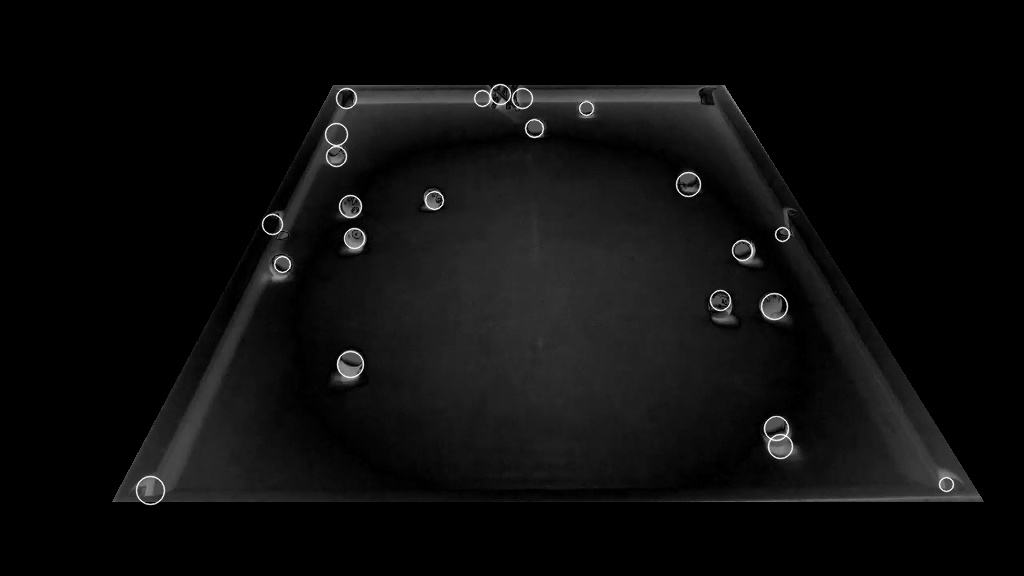
\includegraphics[width=\textwidth]{imgs/ball_localization/circlesHSV.jpg}
        \caption{starting with the HSV version}
    \end{subfigure}
    \caption{Circles detected via HoughCircles on the pre-processed image (game2\_clip1)}
    \label{fig:circles}
\end{figure}

Many balls were detected in both iterations so a smart way to merge the detected circles was necessary.
The final vector of circles is generated by adding all the ones found from the BGR version of the image, that proved 
to represent more accurately the ball contours, and every circles obtained from the HSV version that do not overlap with the ones
in the first set. Figure \ref{fig:circles_final} shows the output of such merge on the previous example. \\
\begin{figure}[h!]
    \centering
    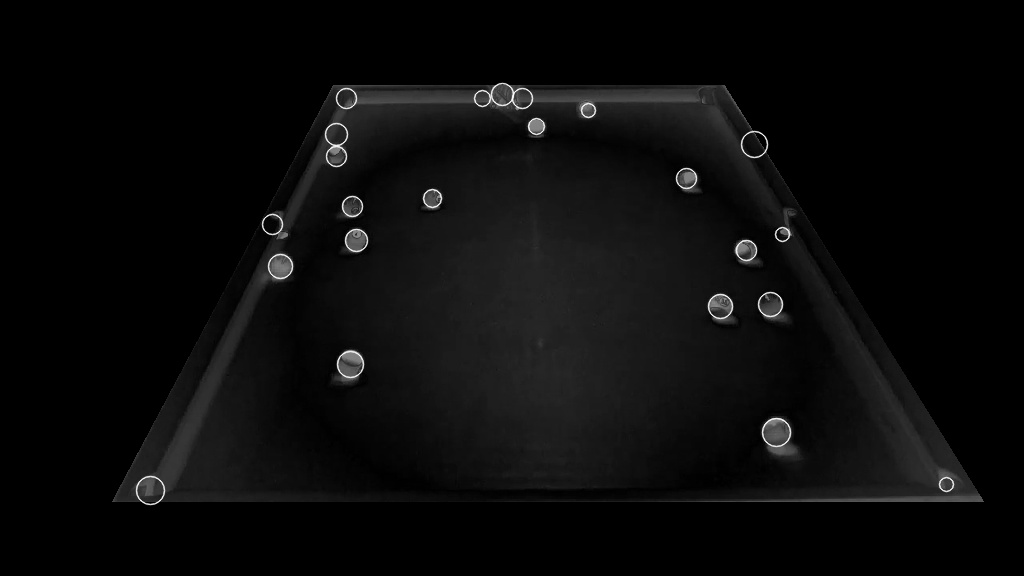
\includegraphics[width=0.85\textwidth]{imgs/ball_localization/circles_merged.jpg}
    \caption{Final set of circles found in the image (game2\_clip1)}
    \label{fig:circles_final}
\end{figure}

Circles were then converted into bounding boxes by creating a Rect object for each circle with abscissa and ordinate equal to the circle ones minus the circle radius,
width and height equal to double the circle radius (diameter).
Through this procedure, for each image a set of bounding boxes is generated, among which exactly one bounding box per ball is contained. 
Figure \ref{fig:fp_detection} shows an example of the results of the procedure upto this point.\\
\begin{figure}[h!]
    \centering
    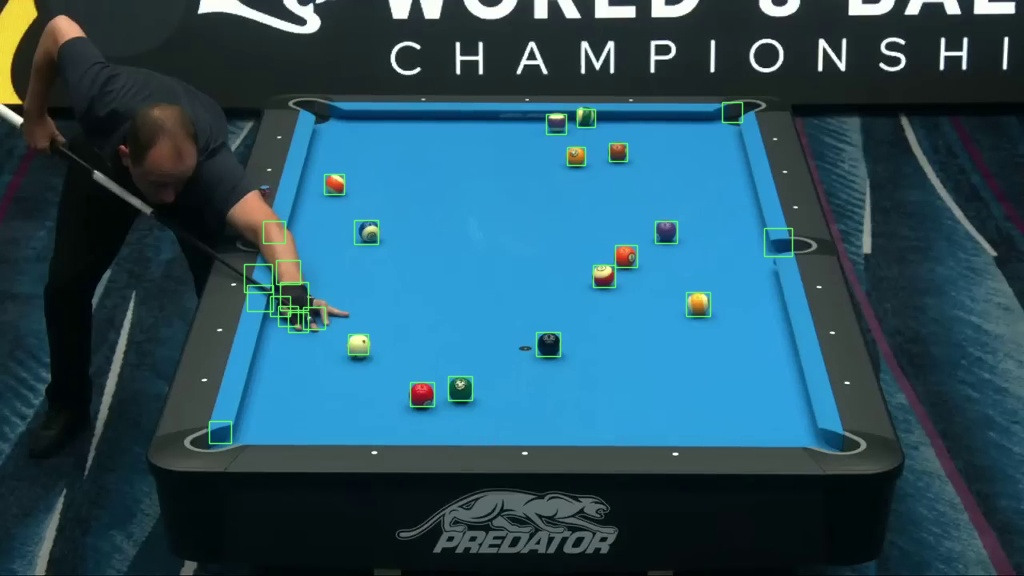
\includegraphics[width=0.85\textwidth]{imgs/ball_localization/fp_detection.jpg}
    \caption{Results of the region proposals generation step (game1\_clip4)}
    \label{fig:fp_detection}
\end{figure}


\subsection{False positive filtering}
As it can be noted from Figure \ref{fig:fp_detection}, to be able to propose regions that cover the whole set of balls in the table, many 
false positive are generated. This happens since there are many circular regions in the table that do not come from any ball.

The first attept at filtering such false positives resulted in the following algorithm. Given the fact that the balls are always inside the table, the surrounding area
of the detected circles (identified as the circular ring of width double the circle diameter and center equal to the circle one) is supposed to have mean intensity similiar to the table 
cloth one and the mean intensity of the area contained in the circle to be different from it. By estimating the table color
and setting proper distance thresholds in the color space, the implemented filter was able to correctly detect most false positives with a few exceptions.
If the player has his arm particulary stretched on the table, circles detected on his hand were detected as true positives and in case of balls touching the table borders with
width almost imperceptible due to perspective effects, the relative circles were detected as false positives.
These errors were caused by the wrong assumptions initially made.

Because of this, other properties of false and true positives were necessary to be identified in order to create an efficient filter.
The found ones are the following.

False positives can belong to either one of the following two classes: circles relative to holes and circles belonging to the player hand and arm if present 
inside the table region. Additionaly, as it will be later better explained, false positives relative to holes are isolated whereas ones relative to the player are always
grouped together. Using these informations, the following algorithm to filter the false positives was created and implemented.

The filter is composed by two sub-filters placed in cascade to detect the false positives.
The first one operates in the following manner. Given the facts that false positive relative to holes can be found on the longest table
borders, and false positives generated by the player are never isolated (distant from other bounding boxes) since
many circles around the arm and hand are always detected, the filter defines an area inside the projection of the table that excludes
the table holes ("safe area") and filters all isolated (non overlapping) bounding boxes which projected center is inside of such area.
To assure that a bounding box is truly isolated, just for this step all boxes width were expanded by a factor $1.5$ so that close but naturally
non-overlapping boxes will now overlap. Figure \ref{fig:safe_area} shows an example of projected table image on which the "safe area" has been drawn.
Note that such rectangle was set at 98\% of the image width and 85\% of its height. These dimensions proved to be effective for the purpose. 
Figure \ref{fig:exp_bboxes} instead shows the result of the bounding boxes expansion applied just for this first filter step. As it can be noticed, close
boxes now overlap, having a better understanding of how much one is isolated.\\
\begin{figure}[h!]
    \centering
    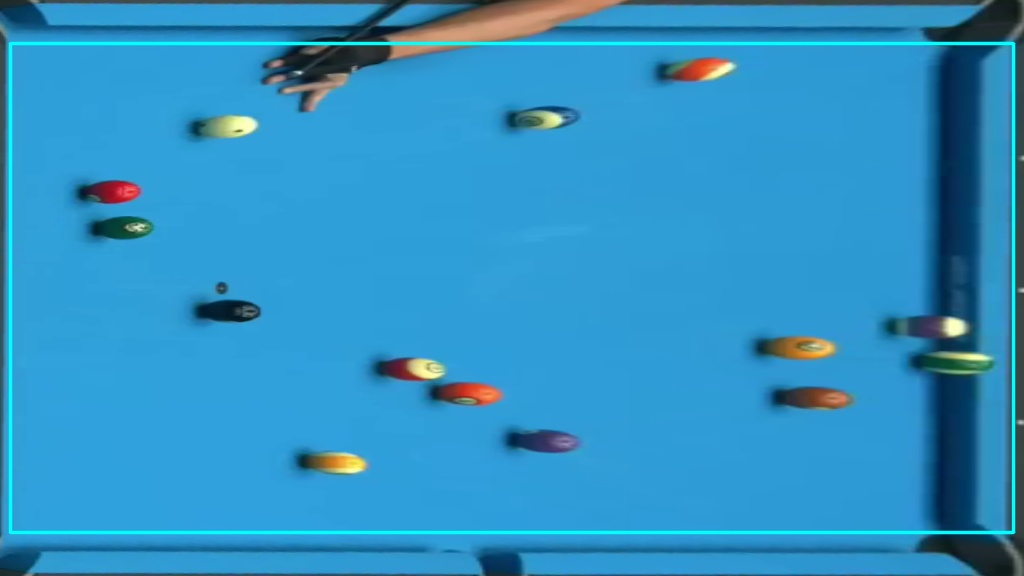
\includegraphics[width=0.85\textwidth]{imgs/ball_localization/safe_area.jpg}
    \caption{Projected table with "safe area" (game1\_clip4)}
    \label{fig:safe_area}
\end{figure}
\begin{figure}[h!]
    \centering
    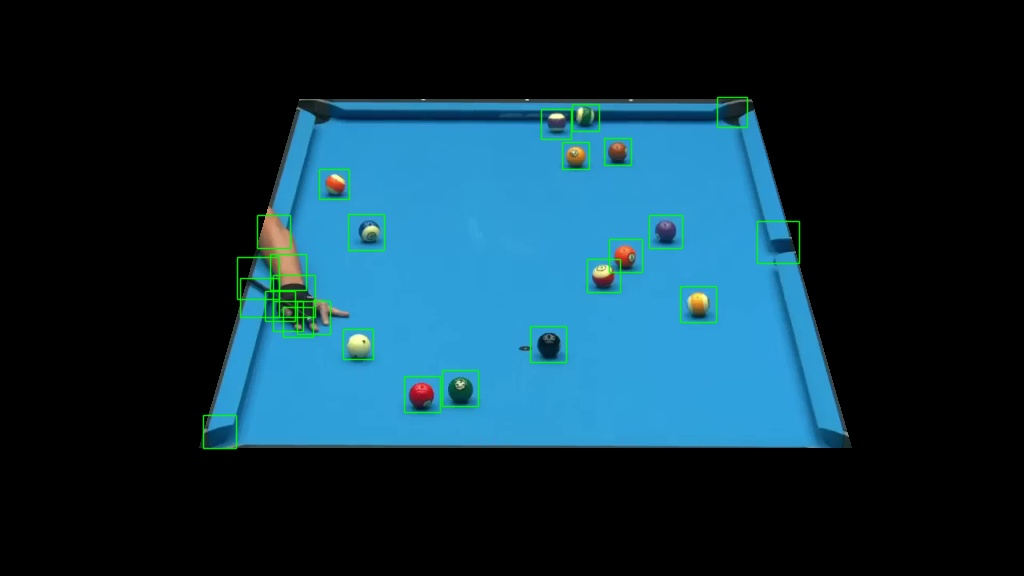
\includegraphics[width=0.85\textwidth]{imgs/ball_localization/exp_boxes_filter.jpg}
    \caption{Expanded bounding boxes in the image (game1\_clip4)}
    \label{fig:exp_bboxes}
\end{figure}

The second and final filter exploits the following property. By dividing the image into connected components, one can notice how found regions belonging to holes, table borders and player arm always
touch the borders of the table projection. This information was exploited to implement the following procedure.
The image is converted in HSV format and the Canny algorithm is applied to the image in order to detect edges.
Then, the projection of the image is obtained using the trasformation matrix returned by the \textit{getTransformation()} function.
This image is then given to the \textit{connectedComponentsWithStats()} method (using Spaghetti labeling algorithm) to obtain
the labeled regions along with useful statistic such the extremal top, bottom, left and right positions of the region.
In this way, a new image is obtained from the transformed canny one by setting at zero all pixels belonging to regions that touch the image
borders or are labeled as background (label 0).
At this point, the percentage of non-zero pixels in each patch of this last image defined by the bounding boxes is computed.
Following our assumptions, all boxes relative to false positives will now contain a low amount of non-zero pixels.
A threshold set at 24\% proved to be effective. Figure \ref{fig:cannyprocess} shows the image resulting from the processing done via \textit{Canny} and \textit{connectedComponentsWithStats}
on which the previously identified bounding boxes are drawn. \\
\begin{figure}[h!]
    \centering
    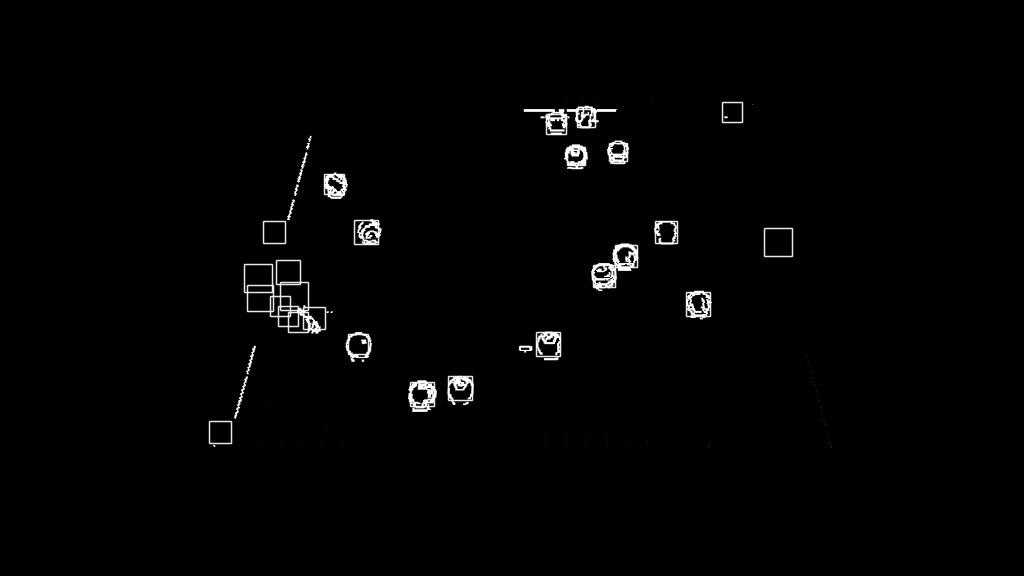
\includegraphics[width=0.85\textwidth]{imgs/ball_localization/conn_comp1.jpg}
    \caption{Results of the canny image processing with bounding boxes (game1\_clip4)}
    \label{fig:cannyprocess}
\end{figure}

Although, this method isn't perfect since it can produce false negatives. In fact, in case of balls close to the borders, their area counted as connected to a component 
of the table border, therefore the respective pixels in the image were set to zero. To fix this kind of errors, a second round of this
procedure is performed but on a new version of the image obtained by running two iterations of the Opening morphological operator with an elliptic 
structuring element of size $(3,2)$. The idea behind this additional step lies in the assumption that table border and balls regions if connected
are weakly connected components. To ensure that no false positive is filtered as true in this last additional step, the percentages
computed during the first iteration are saved into a vector and used during the second in the following manner. If the relative region is no longer touching the image border
and so in the second run the percentage has greatly increased (at least +30\%), then the bounding box is detected as true positive and added
the set of true positives previously computed. Figure \ref{fig:opening} shows an example of this image processing in which when using the Opening operator a ball is disconnected
from the table border and therefore becomes detectable as positive (see the top-left border).\\
\begin{figure}[h!]
    \centering
    \begin{subfigure}[b]{0.85\textwidth}
        \centering
        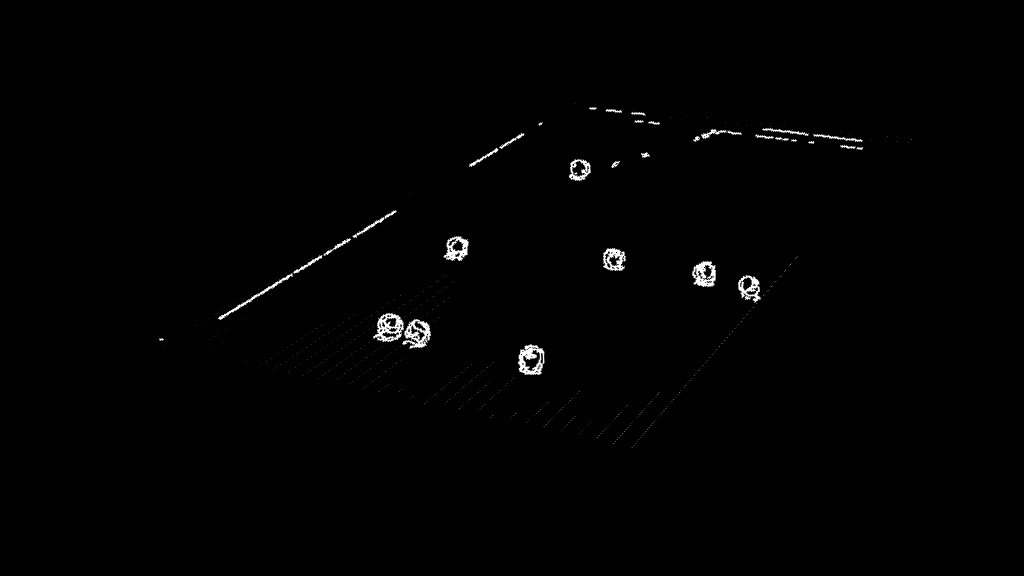
\includegraphics[width=\textwidth]{imgs/ball_localization/final_first.jpg}
        \caption{without Opening (untouched)}
    \end{subfigure}
    % \hspace{0.05\textwidth}
    \\
    \begin{subfigure}[b]{0.85\textwidth}
        \centering
        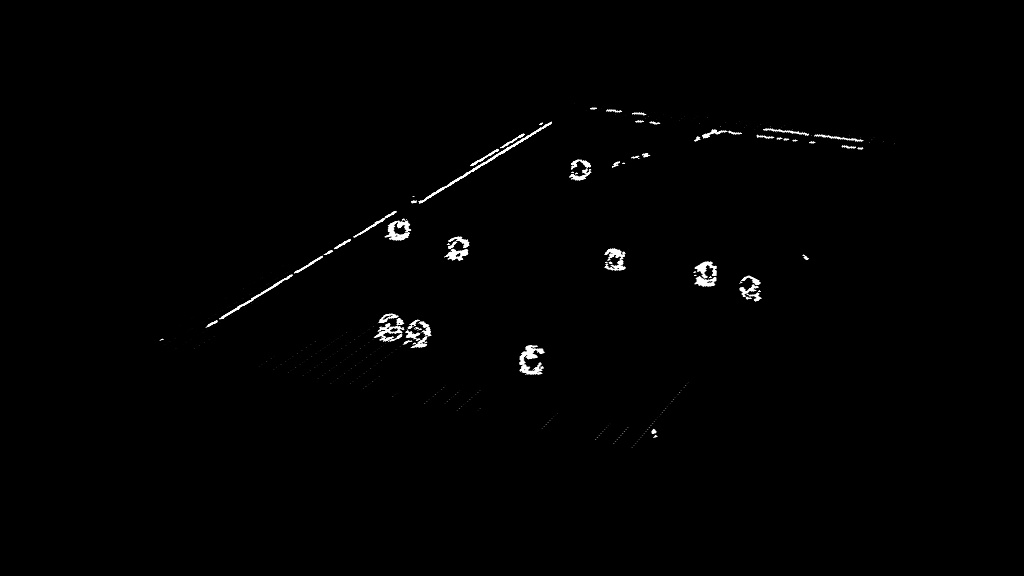
\includegraphics[width=\textwidth]{imgs/ball_localization/final_second.jpg}
        \caption{with Opening (modified)}
    \end{subfigure}
    \caption{Differences in the results of the image processing (game3\_clip1)}
    \label{fig:opening}
\end{figure}

Using this filter, only the regions (bounding boxes) relative to the balls were kept, ensuring a number of false positives and false
negatives equal to zero across the whole provided dataset. Figure \ref{fig:filtering} shows an example of the final results of the complete false positives filtering step of the algorithm.\\
\begin{figure}[h!]
    \centering
    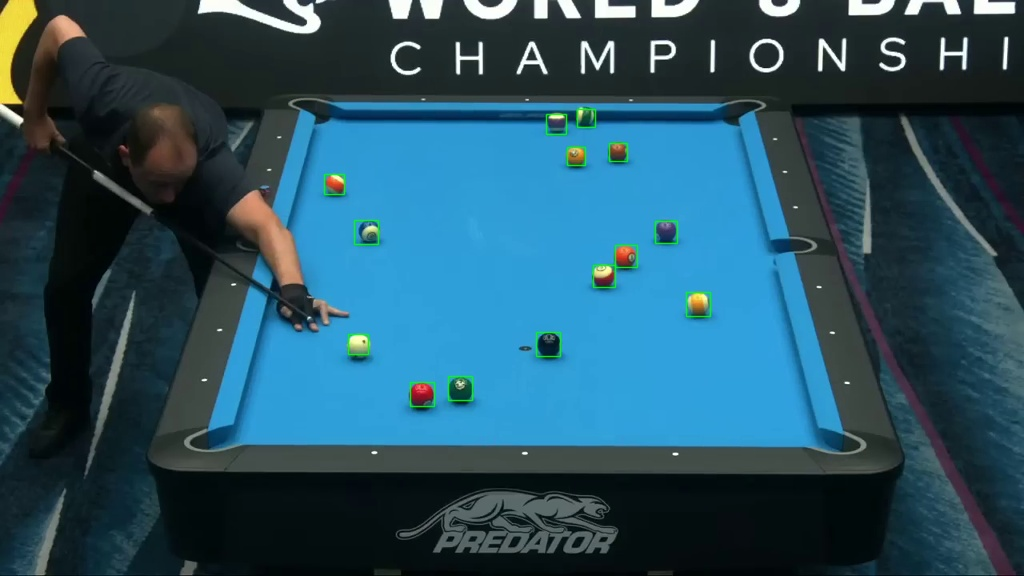
\includegraphics[width=0.85\textwidth]{imgs/ball_localization/filtered_bboxes.jpg}
    \caption{Results of the false positives filtering step (game1\_clip4)}
    \label{fig:filtering}
\end{figure}


\subsection{Bounding boxes refinement}
As suggested by the previous section titles, the found bounding boxes can only be considered as region proposals, since the circles
found through \textit{HoughCircles} in the first step of the detection are not always accurate. This happens because the algorithm was used with a general range of parameters that is supposed to work 
on every possibile image. To obtain the final set of bounding boxes, such regions must be refined.
To do so, we relied once again on \textit{HoughCircles}. To ensure greater precision on the ball circle detection the following operations were carried.
Since in some cases the obtained bounding boxes appeared to be sensibly bigger or smaller than the actual ball shape, to have some reference box dimensions the average
bounding box width was computed. For each box center, a rectangular mask with dimensions equal to the mean box width multiplied by a scaling coefficient (1.1) is applied to 
the image in such point to focus on the surrounding area around of the ball. The scaling is necessary to ensure that the whole ball appears in the mask image, since the previously computed bounding
boxes are often really tight.

After doing so, \textit{GrabCut} algorithm (\textit{grubCut()} in OpenCV) is used to perform foreground extraction in order to obtain an approximate segmentation of the ball in the masked image in HSV format. 
Then, \textit{HoughCircles} is used on the obtained image with the same set of parameters used before with the exception of the accumulator threshold now set at $10$, and
the radius range that now goes from a third to $70\%$ of the mean bounding box width. The choice on this parameters was made to ensure the detection of circles with true ball dimensions
in the specific image, which were estimated through the mean width computation.

This estimation is valid since at most a few boxes have dimensions sensibly different from the true ones. This information is exploited also to ensure that this refinement
does not worsen the quality of already precise bounding boxes. More precisely, only the bounding boxes for which the detected circle has absolute value of difference between radius and previous box
width halfs greater than $4$ are updated. The update is performed by substituting the previous box with the found circle coverted to bounding box in the manner explained before.
Figure \ref{fig:refine} shows an example in which a ball was not precisely detected in the first step and the respective bounding box is refined by the procedure explained in this section. \\
\begin{figure}[h!]
    \centering
    \begin{subfigure}[b]{0.25\textwidth}
        \centering
        
\includegraphics[width=\textwidth]{imgs/ball_localization/bbox_before.jpg}
        \caption{original box}
    \end{subfigure}
    \hspace{0.05\textwidth}
    \begin{subfigure}[b]{0.25\textwidth}
        \centering
        
\includegraphics[width=\textwidth]{imgs/ball_localization/grabcut.jpg}
        \caption{GrabCut output}
    \end{subfigure}
    \hspace{0.05\textwidth}
    \begin{subfigure}[b]{0.25\textwidth}
        \centering
        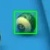
\includegraphics[width=\textwidth]{imgs/ball_localization/bbox_after.jpg}
        \caption{refined box}
    \end{subfigure}
    \caption{Example of bounding box refinement procedure (game1\_clip2)}
    \label{fig:refine}
\end{figure}
It must be noted that sometimes the \textit{GrabCut} algorithm fails to return an accurate ball segmentation since it sometimes considers table borders, holes and shadow of the ball as part of the latter.
In such cases, \textit{HoughCircles} won't find any circles and therefore the relative bounding box won't be updated.
For the same reason, this algorithm is adopted only in this last step and it is not used as backbone of the whole ball localization and segmentation procedure.

\section{Ball Identification (Giacomin Marco)}
TODO

\section{Ball Tracking (Toffolon Mattia)}
\section{Ball Tracking}

To perform the tracking of the balls along the video we decided not to run the ball detection algorithm on each frame since it could generate false positives and negatives.
Instead, we preferred using the \textit{Tracker} classes provided by \textit{OpenCV} that are supposed to provide greater stability and performance with respect to manual detection.
Initially, we adopted the \textit{MultiTracker} class but it didn't provide the level of control we needed. In fact, using such class it was not possibile to distinguish
between tracked balls leading to problems such as not being able to know which ball is lost when the tracker fails. Therefore, we decided to use a vector of single trackers,
each one following a specific ball along the video.
\newline \\
Since the are multiple types of trackers provided by \textit{OpenCV}, a testing phase was needed to understand which one better suited our problem. Firstly, all trackers
relying on Deep Learning were removed from the candidate list since their use is prohibited by the project guidelines. Some tests were run with the remaing ones, and the best tracker,
albeit the one with the longest running time, proved to be \textit{TrackerCSRT}.
\newline \\
Having chose the tracker type, the \textit{TrackBalls} class was created. This class has as attributes a vector of \textit{TrackerCSRT} objects, a vector of \textit{Ball} structs
and an integer constant which use will be later explained. In the following paragraphs the methods of the class and therefore the actual use of the tracker will be presented.
\newline \\
The class constructor takes as parameters a vector of \textit{Ball} structs, which, to recall, are composed by a ball type and a bounding box (Rect object), and the initial frame.
These objects are used to initialize the class attributes. From practical experience we have seen that using tight bounding boxes can sometimes lead to a tracker failing
to recognize the tracked ball between frames. Therefore, before the attributes initialization, the boxes width of the given \textit{Ball} structs are expanded by the constant
previously mentioned. 
\newline \\
To update the trackers and obtain the new state (bounding box position) of the balls, the \textit{update} method was implemented. The latter receives as parameters the next 
video frame and a vector of integers passed by reference which is shared with the renderer. For each tracked ball, the relative tracker is updated using the given frame.
If the tracker peforms such operation succesfully, then the bounding box of the ball is updated only if the intersection over union (IoU) between old and new box is under
the threshold of $0.8$ and the relative box index is added to a specific vector. This condition was set to avoid updates of balls which are still, resulting into a better final video rendering in which only moving balls actually move
and the drawn trajectories are more straight. Instead, if the tracker fails, the ball box isn't updated and the relative index is added into a different vector.
\newline \\
If at the end of the update phase this last vector has positive size, ball recovery operations are carried and if unsuccessful, the relative ball removal from the attributes 
must be carried. Now these steps will be explained. In this case, the ball localization algorithm is run on the new video frame. If the number of detected balls equals the one
of the tracked balls then the recovery of the lost balls can be done. Firstly, for each ball which tracking update was succesfully performed, the closest detected bounding box
is assigned to it and removed from the list of the found ones. Then, the same procedure is carried on the lost balls with the remaining boxes. For each pair of lost ball and box,
the relative tracker and \textit{Ball} struct is re-initialized accordingly.
\newline \\
Instead, in the case in which the localization returns a different number of boxes, the tracking update is declared as failed and the lost balls are deleted. 
The \textit{removeBalls} method was implemented to perform such operation. Using the given vector of indexes representing the list of balls to delete, the respective
tracker and \textit{Ball} struct are erased from the vector attributes.
\newline \\
Additionaly, a \textit{getRealBalls} method was implemented to obtained the de-scaled (true size) bounding box versions of the balls using the same constant adopted in
the constructor. This was useful to obtain the real-size boxes at the end of the tracking, in the last video frame, and therefore to be able to compute correctly
the performances also in such case.

\section{Minimap Rendering (Artico Giovanni)}
\section{Minimap Rendering}

The renderer for the minimap was developed in order for it to use the videoPlayer and 
tracker directly. In order to represent the balls correctly the perspective transformation
matrix, that maps the balls to a predermined rectangle with top left side $(0,0)$. We decided
the dimension of such rectangle to be fixed to $500 \times 1000$ pixels, as the usual ratio
for a billiard table is $1:2$. For the dimension of the balls we used $\frac{1}{70}$ the minimap
columns. This was decided empirically on the videos provided, however such radius does not work
with the same precision on all videos, as there are multiple standards for the billiard table 
dimensions.\par 
For the rendering one buffer is kept for the trajectories, at each frame the line between the
previous and current position is drawn as a black line. this buffer is then copied and the
balls are added. To this the png representing the borders is superimposed (the resizing is hard-coded
as the dimensions are always the same), this needs the executable to be always in the same relative
path as the image is contained in the data folder.\par 
Another role of the render is to determine whether a ball went into a hole or not. We decided to
give this role to the this class, even though architecturally it wouldn't be correct, as it is the 
only one that has both knowledge of the trackers and of the actual positions of the balls on the table.
The method used is to determine the closeness of the center of the bounding box of the ball to one 
of the centers. This verification is done only to balls that have moved in the current frame. The
threshold used is 20 pixels, determined empirically. This method is however not perfect, as the 
tracker may behave unexpectedly when a ball enters a hole, as the object it is tracking is disappearing.
This also is problematic when the hole is occluded by the table border itself, as the tracking may fail
to be precise. Another problem is when a ball is particularly close to a hole but not inside, as it
might be falsely put into a hole. If the renderer detects a ball entering a hole it communicates
this to the tracker which drops the ball.



\section{System Performance Evaluation (Giacomin Marco)}
\label{sec:performance}
% PERFORMANCE MEASURE REPORT
% by Marco Giacomin

\section{System Performance Evaluation}

The project specifications require two distinct performance 
measures to judge the quality of the segmentation produced 
by the program:

\begin{enumerate}
    \item Mean intersection over union (mIoU) for the class segmentation;
    \item Mean average precision (mAP) for ball localization.
\end{enumerate}



\subsection{Intersection over Union (IoU)}

This is the more straightforward of the two measures. 
Given any kind of prediction-truth pairs that represent 
areas (be it a binary mask or a 2d rectangle), the IoU is 
simply the ratio between the area of the intersection of the 
two surfaces and their union.

\begin{figure}[h]
    \centering
    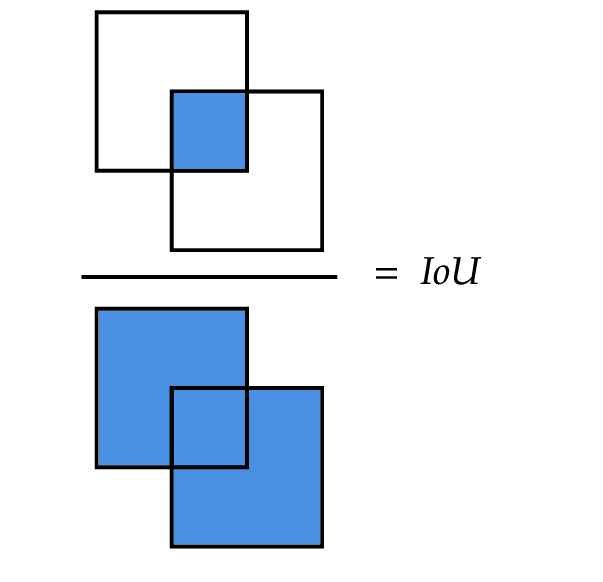
\includegraphics[width=0.4\textwidth]{./imgs/iou.png}
    \caption{Graphical representation of IoU}
\end{figure}

Intuitively, this can be used to represent how well a singular 
prediction in an object detection task fits on the corresponding 
ground truth.
OpenCV provides easy ways to intersect both binary masks and 
\verb|cv::Rect| objects, the first by pixel-wise logical AND 
and the second by a dedicated function.
Union area is instead directly calculated by adding the 
areas of the two surfaces and subtracting the area of 
their intersection.


\subsection{Average precision}

For each ball class for which we make predictions, we are going to 
calculate a metric known as average precision (AP), which is the 
area under the precision-recall curve of the class, per-image, estimated 
using the technique described in the linked article on the project specifications.
For each predicted bounding box, we calculate its maximum IoU with the 
set of ground truths, then we consider it a true positive if the 
value is more than a certain threshold (0.5 in this case). 
We keep a tally of true vs false positives and use it to calculate 
the partial precision and recall values, which we plot in a sparse 
graph (here represented as a \verb|std::map| object).

The area under this graph gives us information on how well the 
localization is performing (1 denotes a perfect classifier, 0 a 
completely wrong one). Since we've build a sparse graph, the 
approximation method PASCAL VOC is used to calculate the 
underlying area: 11 equally spaced points are taken in the 
recall interval (from 0 to 1). For each of those, the corresponding 
precision value is defined as the highest one among all the 
points to the right of it.

\begin{figure}[h]
    \centering
    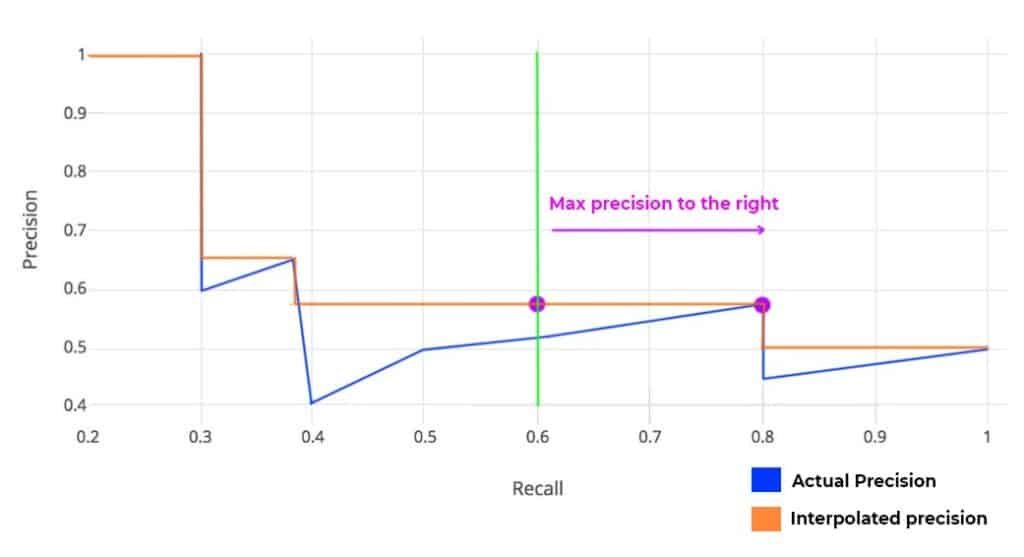
\includegraphics[width=0.8\textwidth]{./imgs/average_precision_graph.jpg}
    \caption{Example of underlying area estimation of a sparse graph}
\end{figure}

The estimation is the average of the 11 values found this way. The "mean" 
in Mean Average Precision is simply the average of all the AP scores 
calculated for each ball class.

In must be noted that in some clips we might have empty classes (for example, an 
endgame position where all the striped balls have been scored). The 
AP for such cases is defined as 1.

\section{Results}
% \section{Results}
In this section the full output of the developed system is presented with the exception of the rendered videos.
For each game event first and last video frames, the generated table and balls segmentation, along with their classification expressed as a color choice,
are presented in form of contours and bounding boxes in the first case, and masks in the second one.
Additionaly, the generated map in its state at the last video frame is reported.
\\
Along with these images, the requested performance metrics were computed and reported in specific tables.
To be more clear, also the intermediate results of the metrics computation are reported.


\begin{figure}
\includegraphics[width=0.49\textwidth]{../samples/sample0/frame_first.png}
\includegraphics[width=0.49\textwidth]{../samples/sample0/frame_last.png}
\newline
\includegraphics[width=0.49\textwidth]{../samples/sample0/output_first.png}
\includegraphics[width=0.49\textwidth]{../samples/sample0/output_last.png}
\newline
\includegraphics[width=0.49\textwidth]{../samples/sample0/output_first_segmentation.png}
\includegraphics[width=0.49\textwidth]{../samples/sample0/output_last_segmentation.png}
\newline
\begin{subfigure}[b]{0.49\textwidth}
    \vspace{20pt}
    \includegraphics[width=\textwidth]{../samples/sample0/predicted_trajectory.png}
    \caption*{game1\_clip1}
\end{subfigure}
\begin{subfigure}[b]{0.49\textwidth}
\begin{tabular}{|l|c|}
    \hline
    \textbf{Metric} & \textbf{Value} \\
    \hline
    Average Precision Localization First & 0.763636 \\
    Average Precision Localization Last & 0.878788 \\
    \hline
    IoU Segmentation Cue First & 0.548523 \\
    IoU Segmentation Cue Last & 0.62069 \\
    IoU Segmentation Eight First & 0.747475 \\
    IoU Segmentation Eight Last & 0.743719 \\
    IoU Segmentation Solid First & 0.53632 \\
    IoU Segmentation Solid Last & 0.536812 \\
    IoU Segmentation Striped First & 0.505707 \\
    IoU Segmentation Striped Last & 0.579247 \\
    \hline
    IoU Table First & 0.957752 \\
    IoU Table Last & 0.968417 \\
    IoU Background First & 0.969238 \\
    IoU Background Last & 0.977193 \\
    \hline
    Average Precision Cue First & 1 \\
    Average Precision Cue Last & 1 \\
    Average Precision Eight First & 1 \\
    Average Precision Eight Last & 1 \\
    Average Precision Solid First & 0.818182 \\
    Average Precision Solid Last & 0.818182 \\
    Average Precision Striped First & 0.620779 \\
    Average Precision Striped Last & 0.74026 \\
    \hline
    mIOU First & 0.710836 \\
    mIOU Last & 0.73768 \\
    mAP First & 0.85974 \\
    mAP Last & 0.88961 \\
    \hline
\end{tabular}
\end{subfigure}
\end{figure}

\begin{figure}
    \includegraphics[width=0.49\textwidth]{../samples/sample1/frame_first.png}
    \includegraphics[width=0.49\textwidth]{../samples/sample1/frame_last.png}
    \newline
    \includegraphics[width=0.49\textwidth]{../samples/sample1/output_first.png}
    \includegraphics[width=0.49\textwidth]{../samples/sample1/output_last.png}
    \newline
    \includegraphics[width=0.49\textwidth]{../samples/sample1/output_first_segmentation.png}
    \includegraphics[width=0.49\textwidth]{../samples/sample1/output_last_segmentation.png}
    \newline
    \begin{subfigure}[b]{0.49\textwidth}
        \vspace{20pt}
        \includegraphics[width=\textwidth]{../samples/sample1/predicted_trajectory.png}
        \caption*{game1\_clip2}
    \end{subfigure}
\begin{subfigure}[b]{0.49\textwidth}
    \begin{tabular}{|l|c|}
        \hline
        \textbf{Metric} & \textbf{Value} \\
        \hline
        Average Precision Localization First & 1 \\
        Average Precision Localization Last & 1 \\
        \hline
        IoU Segmentation Cue First & 0.890208 \\
        IoU Segmentation Cue Last & 0.745263 \\
        IoU Segmentation Eight First & 0.901124 \\
        IoU Segmentation Eight Last & 0.905405 \\
        IoU Segmentation Solid First & 0.379076 \\
        IoU Segmentation Solid Last & 0.329148 \\
        IoU Segmentation Striped First & 0.36483 \\
        IoU Segmentation Striped Last & 0.340779 \\
        \hline
        IoU Table First & 0.945966 \\
        IoU Table Last & 0.956962 \\
        IoU Background First & 0.978064 \\
        IoU Background Last & 0.983876 \\
        \hline
        Average Precision Cue First & 1 \\
        Average Precision Cue Last & 1 \\
        Average Precision Eight First & 1 \\
        Average Precision Eight Last & 1 \\
        Average Precision Solid First & 0.597403 \\
        Average Precision Solid Last & 0.597403 \\
        Average Precision Striped First & 0.454545 \\
        Average Precision Striped Last & 0.454545 \\
        \hline
        mIOU First & 0.743211 \\
        mIOU Last & 0.710239 \\
        mAP First & 0.762987 \\
        mAP Last & 0.762987 \\
        \hline
    \end{tabular}    
\end{subfigure}
\end{figure}

\begin{figure}
    \includegraphics[width=0.49\textwidth]{../samples/sample2/frame_first.png}
    \includegraphics[width=0.49\textwidth]{../samples/sample2/frame_last.png}
    \newline
    \includegraphics[width=0.49\textwidth]{../samples/sample2/output_first.png}
    \includegraphics[width=0.49\textwidth]{../samples/sample2/output_last.png}
    \newline
    \includegraphics[width=0.49\textwidth]{../samples/sample2/output_first_segmentation.png}
    \includegraphics[width=0.49\textwidth]{../samples/sample2/output_last_segmentation.png}
    \newline
    \begin{subfigure}[b]{0.49\textwidth}
        \vspace{20pt}
        \includegraphics[width=\textwidth]{../samples/sample2/predicted_trajectory.png}
        \caption*{game1\_clip3}
    \end{subfigure}
\begin{subfigure}[b]{0.49\textwidth}
    \begin{tabular}{|l|c|}
        \hline
        \textbf{Metric} & \textbf{Value} \\
        \hline
        Average Precision Localization First & 1 \\
        Average Precision Localization Last & 0.606061 \\
        \hline
        IoU Segmentation Cue First & 0.566092 \\
        IoU Segmentation Cue Last & 0.441704 \\
        IoU Segmentation Eight First & 0.748538 \\
        IoU Segmentation Eight Last & 0.749511 \\
        IoU Segmentation Solid First & 0.522388 \\
        IoU Segmentation Solid Last & 0.379761 \\
        IoU Segmentation Striped First & 0.39342 \\
        IoU Segmentation Striped Last & 0.395045 \\
        \hline
        IoU Table First & 0.954457 \\
        IoU Table Last & 0.958917 \\
        IoU Background First & 0.980998 \\
        IoU Background Last & 0.983055 \\
        \hline
        Average Precision Cue First & 1 \\
        Average Precision Cue Last & 0 \\
        Average Precision Eight First & 1 \\
        Average Precision Eight Last & 1 \\
        Average Precision Solid First & 0.666667 \\
        Average Precision Solid Last & 0.5 \\
        Average Precision Striped First & 0.636364 \\
        Average Precision Striped Last & 0.363636 \\
        \hline
        mIOU First & 0.694316 \\
        mIOU Last & 0.651332 \\
        mAP First & 0.825758 \\
        mAP Last & 0.465909 \\
        \hline
    \end{tabular}    
\end{subfigure}
\end{figure}

\begin{figure}
    \includegraphics[width=0.49\textwidth]{../samples/sample3/frame_first.png}
    \includegraphics[width=0.49\textwidth]{../samples/sample3/frame_last.png}
    \newline
    \includegraphics[width=0.49\textwidth]{../samples/sample3/output_first.png}
    \includegraphics[width=0.49\textwidth]{../samples/sample3/output_last.png}
    \newline
    \includegraphics[width=0.49\textwidth]{../samples/sample3/output_first_segmentation.png}
    \includegraphics[width=0.49\textwidth]{../samples/sample3/output_last_segmentation.png}
    \newline
    \begin{subfigure}[b]{0.49\textwidth}
        \vspace{20pt}
        \includegraphics[width=\textwidth]{../samples/sample3/predicted_trajectory.png}
        \caption*{game1\_clip4}
    \end{subfigure}
\begin{subfigure}[b]{0.49\textwidth}
    \begin{tabular}{|l|c|}
        \hline
        \textbf{Metric} & \textbf{Value} \\
        \hline
        Average Precision Localization First & 1 \\
        Average Precision Localization Last & 0.902597 \\
        \hline
        IoU Segmentation Cue First & 0.601518 \\
        IoU Segmentation Cue Last & 0.477358 \\
        IoU Segmentation Eight First & 0.848723 \\
        IoU Segmentation Eight Last & 0.859406 \\
        IoU Segmentation Solid First & 0.549807 \\
        IoU Segmentation Solid Last & 0.535469 \\
        IoU Segmentation Striped First & 0.516323 \\
        IoU Segmentation Striped Last & 0.525094 \\
        \hline
        IoU Table First & 0.921017 \\
        IoU Table Last & 0.945411 \\
        IoU Background First & 0.967132 \\
        IoU Background Last & 0.977882 \\
        \hline
        Average Precision Cue First & 1 \\
        Average Precision Cue Last & 0 \\
        Average Precision Eight First & 1 \\
        Average Precision Eight Last & 1 \\
        Average Precision Solid First & 0.772727 \\
        Average Precision Solid Last & 0.772727 \\
        Average Precision Striped First & 0.636364 \\
        Average Precision Striped Last & 0.636364 \\
        \hline
        mIOU First & 0.734087 \\
        mIOU Last & 0.720103 \\
        mAP First & 0.852273 \\
        mAP Last & 0.602273 \\
        \hline
    \end{tabular}    
\end{subfigure}
\end{figure}

\begin{figure}
    \includegraphics[width=0.49\textwidth]{../samples/sample4/frame_first.png}
    \includegraphics[width=0.49\textwidth]{../samples/sample4/frame_last.png}
    \newline
    \includegraphics[width=0.49\textwidth]{../samples/sample4/output_first.png}
    \includegraphics[width=0.49\textwidth]{../samples/sample4/output_last.png}
    \newline
    \includegraphics[width=0.49\textwidth]{../samples/sample4/output_first_segmentation.png}
    \includegraphics[width=0.49\textwidth]{../samples/sample4/output_last_segmentation.png}
    \newline
    \begin{subfigure}[b]{0.49\textwidth}
        \vspace{20pt}
        \includegraphics[width=\textwidth]{../samples/sample4/predicted_trajectory.png}
        \caption*{game2\_clip1}
    \end{subfigure}
\begin{subfigure}[b]{0.49\textwidth}
    \begin{tabular}{|l|c|}
        \hline
        \textbf{Metric} & \textbf{Value} \\
        \hline
        Average Precision Localization First & 0.833333 \\
        Average Precision Localization Last & 0.833333 \\
        \hline
        IoU Segmentation Cue First & 0.828571 \\
        IoU Segmentation Cue Last & 0.837349 \\
        IoU Segmentation Eight First & 0 \\
        IoU Segmentation Eight Last & 0 \\
        IoU Segmentation Solid First & 0.230531 \\
        IoU Segmentation Solid Last & 0.243353 \\
        IoU Segmentation Striped First & 0.41396 \\
        IoU Segmentation Striped Last & 0.42682 \\
        \hline
        IoU Table First & 0.973516 \\
        IoU Table Last & 0.968534 \\
        IoU Background First & 0.98538 \\
        IoU Background Last & 0.981183 \\
        \hline
        Average Precision Cue First & 1 \\
        Average Precision Cue Last & 1 \\
        Average Precision Eight First & 0 \\
        Average Precision Eight Last & 0 \\
        Average Precision Solid First & 0.272727 \\
        Average Precision Solid Last & 0.272727 \\
        Average Precision Striped First & 0.6 \\
        Average Precision Striped Last & 0.6 \\
        \hline
        mIOU First & 0.571993 \\
        mIOU Last & 0.576207 \\
        mAP First & 0.468182 \\
        mAP Last & 0.468182 \\
        \hline
    \end{tabular}
    
\end{subfigure}
\end{figure}

\begin{figure}
    \includegraphics[width=0.49\textwidth]{../samples/sample5/frame_first.png}
    \includegraphics[width=0.49\textwidth]{../samples/sample5/frame_last.png}
    \newline
    \includegraphics[width=0.49\textwidth]{../samples/sample5/output_first.png}
    \includegraphics[width=0.49\textwidth]{../samples/sample5/output_last.png}
    \newline
    \includegraphics[width=0.49\textwidth]{../samples/sample5/output_first_segmentation.png}
    \includegraphics[width=0.49\textwidth]{../samples/sample5/output_last_segmentation.png}
    \newline
    \begin{subfigure}[b]{0.49\textwidth}
        \vspace{20pt}
        \includegraphics[width=\textwidth]{../samples/sample5/predicted_trajectory.png}
        \caption*{game2\_clip2}
    \end{subfigure}
\begin{subfigure}[b]{0.49\textwidth}
    \begin{tabular}{|l|c|}
        \hline
        \textbf{Metric} & \textbf{Value} \\
        \hline
        Average Precision Localization First & 1 \\
        Average Precision Localization Last & 0.909091 \\
        \hline
        IoU Segmentation Cue First & 0.727612 \\
        IoU Segmentation Cue Last & 0.370301 \\
        IoU Segmentation Eight First & 0 \\
        IoU Segmentation Eight Last & 0 \\
        IoU Segmentation Solid First & 0.511984 \\
        IoU Segmentation Solid Last & 0.420787 \\
        IoU Segmentation Striped First & 0.653567 \\
        IoU Segmentation Striped Last & 0.652642 \\
        \hline
        IoU Table First & 0.973231 \\
        IoU Table Last & 0.972855 \\
        IoU Background First & 0.982659 \\
        IoU Background Last & 0.984523 \\
        \hline
        Average Precision Cue First & 1 \\
        Average Precision Cue Last & 0 \\
        Average Precision Eight First & 0 \\
        Average Precision Eight Last & 0 \\
        Average Precision Solid First & 0.636364 \\
        Average Precision Solid Last & 0.545455 \\
        Average Precision Striped First & 0.924242 \\
        Average Precision Striped Last & 0.924242 \\
        \hline
        mIOU First & 0.641509 \\
        mIOU Last & 0.566851 \\
        mAP First & 0.640152 \\
        mAP Last & 0.367424 \\
        \hline
    \end{tabular}    
\end{subfigure}
\end{figure}

\begin{figure}
    \includegraphics[width=0.49\textwidth]{../samples/sample6/frame_first.png}
    \includegraphics[width=0.49\textwidth]{../samples/sample6/frame_last.png}
    \newline
    \includegraphics[width=0.49\textwidth]{../samples/sample6/output_first.png}
    \includegraphics[width=0.49\textwidth]{../samples/sample6/output_last.png}
    \newline
    \includegraphics[width=0.49\textwidth]{../samples/sample6/output_first_segmentation.png}
    \includegraphics[width=0.49\textwidth]{../samples/sample6/output_last_segmentation.png}
    \newline
    \begin{subfigure}[b]{0.49\textwidth}
        \vspace{20pt}
        \includegraphics[width=\textwidth]{../samples/sample6/predicted_trajectory.png}
        \caption*{game3\_clip1}
    \end{subfigure}
\begin{subfigure}[b]{0.49\textwidth}
    \begin{tabular}{|l|c|}
        \hline
        \textbf{Metric} & \textbf{Value} \\
        \hline
        Average Precision Localization First & 1 \\
        Average Precision Localization Last & 0.806818 \\
        \hline
        IoU Segmentation Cue First & 0.562264 \\
        IoU Segmentation Cue Last & 0.351415 \\
        IoU Segmentation Eight First & 0.693182 \\
        IoU Segmentation Eight Last & 0.696275 \\
        IoU Segmentation Solid First & 0.588556 \\
        IoU Segmentation Solid Last & 0.545855 \\
        IoU Segmentation Striped First & 0.537661 \\
        IoU Segmentation Striped Last & 0.542875 \\
        \hline
        IoU Table First & 0.954921 \\
        IoU Table Last & 0.968478 \\
        IoU Background First & 0.988175 \\
        IoU Background Last & 0.992289 \\
        \hline
        Average Precision Cue First & 1 \\
        Average Precision Cue Last & 0 \\
        Average Precision Eight First & 1 \\
        Average Precision Eight Last & 1 \\
        Average Precision Solid First & 1 \\
        Average Precision Solid Last & 1 \\
        Average Precision Striped First & 0.727273 \\
        Average Precision Striped Last & 0.727273 \\
        \hline
        mIOU First & 0.720793 \\
        mIOU Last & 0.682864 \\
        mAP First & 0.931818 \\
        mAP Last & 0.681818 \\
        \hline
    \end{tabular}    
\end{subfigure}
\end{figure}

\begin{figure}
    \includegraphics[width=0.49\textwidth]{../samples/sample7/frame_first.png}
    \includegraphics[width=0.49\textwidth]{../samples/sample7/frame_last.png}
    \newline
    \includegraphics[width=0.49\textwidth]{../samples/sample7/output_first.png}
    \includegraphics[width=0.49\textwidth]{../samples/sample7/output_last.png}
    \newline
    \includegraphics[width=0.49\textwidth]{../samples/sample7/output_first_segmentation.png}
    \includegraphics[width=0.49\textwidth]{../samples/sample7/output_last_segmentation.png}
    \newline
    \begin{subfigure}[b]{0.49\textwidth}
        \vspace{20pt}
        \includegraphics[width=\textwidth]{../samples/sample7/predicted_trajectory.png}
        \caption*{game3\_clip2}
    \end{subfigure}
\begin{subfigure}[b]{0.49\textwidth}
    \begin{tabular}{|l|c|}
        \hline
        \textbf{Metric} & \textbf{Value} \\
        \hline
        Average Precision Localization First & 1 \\
        Average Precision Localization Last & 1 \\
        \hline
        IoU Segmentation Cue First & 0.759804 \\
        IoU Segmentation Cue Last & 0.749361 \\
        IoU Segmentation Eight First & 0.6875 \\
        IoU Segmentation Eight Last & 0.685637 \\
        IoU Segmentation Solid First & 0.209217 \\
        IoU Segmentation Solid Last & 0.148784 \\
        IoU Segmentation Striped First & 0.151724 \\
        IoU Segmentation Striped Last & 0.154028 \\
        \hline
        IoU Table First & 0.945646 \\
        IoU Table Last & 0.948466 \\
        IoU Background First & 0.985851 \\
        IoU Background Last & 0.986169 \\
        \hline
        Average Precision Cue First & 1 \\
        Average Precision Cue Last & 1 \\
        Average Precision Eight First & 1 \\
        Average Precision Eight Last & 1 \\
        Average Precision Solid First & 0.290909 \\
        Average Precision Solid Last & 0.272727 \\
        Average Precision Striped First & 0.242424 \\
        Average Precision Striped Last & 0.242424 \\
        \hline
        mIOU First & 0.62329 \\
        mIOU Last & 0.612074 \\
        mAP First & 0.633333 \\
        mAP Last & 0.628788 \\
        \hline
    \end{tabular}
    
\end{subfigure}
\end{figure}

\begin{figure}
    \includegraphics[width=0.49\textwidth]{../samples/sample8/frame_first.png}
    \includegraphics[width=0.49\textwidth]{../samples/sample8/frame_last.png}
    \newline
    \includegraphics[width=0.49\textwidth]{../samples/sample8/output_first.png}
    \includegraphics[width=0.49\textwidth]{../samples/sample8/output_last.png}
    \newline
    \includegraphics[width=0.49\textwidth]{../samples/sample8/output_first_segmentation.png}
    \includegraphics[width=0.49\textwidth]{../samples/sample8/output_last_segmentation.png}
    \newline
    \begin{subfigure}[b]{0.49\textwidth}
        \vspace{20pt}
        \includegraphics[width=\textwidth]{../samples/sample8/predicted_trajectory.png}
        \caption*{game4\_clip1}
    \end{subfigure}
\begin{subfigure}[b]{0.49\textwidth}
    \begin{tabular}{|l|c|}
        \hline
        \textbf{Metric} & \textbf{Value} \\
        \hline
        Average Precision Localization First & 1 \\
        Average Precision Localization Last & 1 \\
        \hline
        IoU Segmentation Cue First & 0 \\
        IoU Segmentation Cue Last & 0 \\
        IoU Segmentation Eight First & 0.866044 \\
        IoU Segmentation Eight Last & 0.858934 \\
        IoU Segmentation Solid First & 0 \\
        IoU Segmentation Solid Last & 0 \\
        IoU Segmentation Striped First & 0.369556 \\
        IoU Segmentation Striped Last & 0.415295 \\
        \hline
        IoU Table First & 0.965927 \\
        IoU Table Last & 0.975223 \\
        IoU Background First & 0.984447 \\
        IoU Background Last & 0.989119 \\
        \hline
        Average Precision Cue First & 0 \\
        Average Precision Cue Last & 0 \\
        Average Precision Eight First & 1 \\
        Average Precision Eight Last & 1 \\
        Average Precision Solid First & 0 \\
        Average Precision Solid Last & 0 \\
        Average Precision Striped First & 0.484848 \\
        Average Precision Striped Last & 0.545455 \\
        \hline
        mIOU First & 0.530996 \\
        mIOU Last & 0.539762 \\
        mAP First & 0.371212 \\
        mAP Last & 0.386364 \\
        \hline
    \end{tabular}    
\end{subfigure}
\end{figure}

\begin{figure}
    \includegraphics[width=0.49\textwidth]{../samples/sample9/frame_first.png}
    \includegraphics[width=0.49\textwidth]{../samples/sample9/frame_last.png}
    \newline
    \includegraphics[width=0.49\textwidth]{../samples/sample9/output_first.png}
    \includegraphics[width=0.49\textwidth]{../samples/sample9/output_last.png}
    \newline
    \includegraphics[width=0.49\textwidth]{../samples/sample9/output_first_segmentation.png}
    \includegraphics[width=0.49\textwidth]{../samples/sample9/output_last_segmentation.png}
    \newline
    \begin{subfigure}[b]{0.49\textwidth}
        \vspace{20pt}
        \includegraphics[width=\textwidth]{../samples/sample9/predicted_trajectory.png}
        \caption*{game4\_clip2}
    \end{subfigure}
\begin{subfigure}[b]{0.49\textwidth}
    \begin{tabular}{|l|c|}
        \hline
        \textbf{Metric} & \textbf{Value} \\
        \hline
        Average Precision Localization First & 1 \\
        Average Precision Localization Last & 0.871212 \\
        \hline
        IoU Segmentation Cue First & 0.702899 \\
        IoU Segmentation Cue Last & 0.711191 \\
        IoU Segmentation Eight First & 0.61442 \\
        IoU Segmentation Eight Last & 0.609375 \\
        IoU Segmentation Solid First & 0.489948 \\
        IoU Segmentation Solid Last & 0.498001 \\
        IoU Segmentation Striped First & 0.448905 \\
        IoU Segmentation Striped Last & 0.391053 \\
        \hline
        IoU Table First & 0.952201 \\
        IoU Table Last & 0.976351 \\
        IoU Background First & 0.97856 \\
        IoU Background Last & 0.990622 \\
        \hline
        Average Precision Cue First & 1 \\
        Average Precision Cue Last & 1 \\
        Average Precision Eight First & 1 \\
        Average Precision Eight Last & 1 \\
        Average Precision Solid First & 0.727273 \\
        Average Precision Solid Last & 0.727273 \\
        Average Precision Striped First & 0.848485 \\
        Average Precision Striped Last & 0.5 \\
        \hline
        mIOU First & 0.697822 \\
        mIOU Last & 0.696099 \\
        mAP First & 0.893939 \\
        mAP Last & 0.806818 \\
        \hline
    \end{tabular}    
\end{subfigure}
\end{figure}

\section{Project Structure}
\section{Project Structure and Execution Instructions}


The project has been developed using the CMake build system and it is organized with the
following structure:
\begin{itemize}
    \item \verb|include| directory, contains the header source code files;
    \item \verb|src| directory, contains the implementation source code files;
    \item \verb|data| directory, contains the background image used to generate the 2D map;
    \item \verb|samples.zip| file, contains the system input, outputs, predictions and ground truths;
    \item \verb|output_videos.zip| file, contains the produced video renderings;
    \item \verb|CMakeLists.txt|, contains CMake instructions to organize the build of the project. 
\end{itemize}

\noindent
The \verb|sample| directory is structured into \verb|samplei| subfolders, where \verb|i| refers to the sample index (starting from zero).
As mentioned before, each subfolder contains inputs, outputs, prediction and ground truths relative to a specific sample.
\\
\noindent
Furthermore, folders \verb|include| and \verb|src| are further divided into:
\begin{itemize}
    \item \verb|segment| directory, contains the files for table and balls segmentatation;
    \item \verb|recognition| directory, contains the files for balls identification and side recognition;
    \item \verb|tracking| directory, contains the files for balls tracking;
    \item \verb|rendering| directory, contains the files for the map rendering;
    \item \verb|utils| directory, contains additional files that implement various utilities.
\end{itemize}

\noindent
Additionaly, \verb|src| folder contains:
\begin{itemize}
    \item \verb|output_main.cpp| file, implements the full video rendering and masks generation;
    \item \verb|performance_main.cpp|, implements the computation of all performance metrics across all videos.
\end{itemize}

\noindent
After successfully build the project using CMake, the two \textit{mains} can be executed under the following conditions.
\verb|output_main.cpp| requires the following three parameters as argument:
\begin{enumerate}
    \item path to the \verb|.mp4| file corresponding to the video;
    \item path to the \verb|.png| file corresponding to the first video frame;
    \item path to the folder in which the program output shall be saved.
\end{enumerate}

\noindent
\verb|performance_main.cpp| instead, requires the following parameters:
\begin{enumerate}
    \item path to the \verb|samples| folder;
    \item total number of samples in the folder.
\end{enumerate}
\verb|sample| is provided in \verb|.zip| format for convenience. Therefore, in order to run the respective executable
successfully, the \verb|.zip| file must be extracted.


\section{Experimental Setup}
The system has been tested under the following environment:
\begin{itemize}
    \item C++ 14.1.1;
    \item CMake 3.30.0;
    \item OpenCV 4.10.0-3;
    \item Linux 6.9.9;
    \item Intel i5 6200u, 8GB RAM.
\end{itemize}

\section{Work Split}
\section{Workload Split}


% \begin{tabular}{ |p{6cm}||p{3cm}|  }
%  \hline
%  \multicolumn{2}{|c|}{Project} \\
%  \hline
%  Task & Owner of task \\
%  \hline
%  Table Segmentation   & Giovanni Artico\\
%  \hline
%  Table Sides Recognition &  Giovanni Artico\\
%  \hline
%  Balls localization and segmentation & Mattia Toffolon\\
%  \hline
%  Balls classification & Marco Giacomin\\
%  \hline
%  Minimap Rendering & Giovanni Artico\\
%  \hline
%  System Performance evaluation & Marco Giacomin\\
%  \hline
%  Ball Tracking architecture and algorithm selection & Giovanni Artico\\
%  \hline
%  Ball Tracking refinement & Mattia Toffolon\\
%  \hline
% \end{tabular}
% \par
% The report was written by the person owner of the task, apart from
% the into section written by Mattia Toffolon.

In this Section, how the workload was split between the authors is shown along with the amount of working hours spent by each one.

The following table associates each identified task with an author. Each author was responsibile for the creation and development of the owned tasks solution.
In some cases, minor contributions in terms of ideas were given by authors different than the task owner.
\begin{table}[h]
\centering
\begin{tabular}{|l|c|c|}
    \hline
    \textbf{Task} & \textbf{Owner} & \textbf{Minor contributors}  \\ \hline
    \\[-1em]
    Table Segmentation  & Giovanni Artico & \\ \hline
    \\[-1em]
    Table Sides Recognition &  Giovanni Artico & \\ \hline
    \\[-1em]
    Balls Localization and Segmentation & Mattia Toffolon & Giovanni Artico\\ \hline
    \\[-1em]
    Balls Classification & Marco Giacomin & \\ \hline
    \\[-1em]
    Balls Tracking & Mattia Toffolon & Giovanni Artico\\ \hline
    \\[-1em]
    Map Rendering & Giovanni Artico & Mattia Toffolon \\ \hline
    \\[-1em]
    System Performance Evaluation & Marco Giacomin & Giovanni Artico \\ \hline
\end{tabular}
\caption{Table representing the workload split among the authors}
\end{table}

\begin{flushleft}
For what concerns the production of the project report, each author was responsibile for the writing of the sections relative to the owned tasks. \\   
\end{flushleft}
The writing of the remaing section was split in the following manner.
Sections: Introduction, Project structure, Experimental setup, Workload split, Conclusions and Future work, were written by Mattia Toffolon. 
Section: Results, was written by Giovanni Artico. \\

\begin{flushleft}
The amount of working hours spent on the project (code plus report) spent by each author is represented in the following table.
\end{flushleft}
\begin{table}[h]
    \centering
    \begin{tabular}{|l|c|}
        \hline
        \textbf{Author} & \textbf{Working Hours} \\ \hline
        \\[-1em]
        Giovanni Artico & \\ \hline
        \\[-1em]
        Marco Giacomin & 28 \\ \hline
        \\[-1em]
        Mattia Toffolon & \\ \hline
    \end{tabular}
    \caption{Table representing the amount of working hours spent by each author}
\end{table}

\section{Conclusions}
\section{Conclusions and Future Work}


The developed system has achieved satisfactory performance in segmentatation of table, balls, background and balls localization, especially considering 
that it is exploiting only traditional computer vision techniques without the use of Machine Learning or Deep Learning.
The ball classification step instead, showed major flaws in multiple cases, bringing down the complexive system performance. 
Despite this, the generated 2D maps proved to represent fairly well the game events on each frame, leading to the creation of a modified version
of the given videos in which useful informations are shown. 
\newline \\
To improve the system, every sub-task solution could be refined.
Other than that, another possibile way in which the project solution could be further improved is the adaptation to live-streaming billiard games. In this case the program should be modified
in order to process the video frames in real-time. Additionaly, in order not to lose any frame, strict time constraints on the images processing shall be added. 

\end{document}
